\documentclass[11pt]{article}
\usepackage[utf8]{inputenc}	% Para caracteres en español
\usepackage{amsmath,amsthm,amsfonts,amssymb,amscd}
\usepackage{multirow,booktabs}
\usepackage[table]{xcolor}
\usepackage{fullpage}
\usepackage{lastpage}
\usepackage{enumitem}
\usepackage{fancyhdr}
\usepackage{mathrsfs}
\usepackage{wrapfig}
\usepackage{setspace}
\usepackage{calc}
\usepackage{multicol}
\usepackage{cancel}
\usepackage[retainorgcmds]{IEEEtrantools}
\usepackage[margin=3cm]{geometry}
\usepackage{amsmath}
\newlength{\tabcont}
\setlength{\parindent}{0.0in}
\setlength{\parskip}{0.05in}
\usepackage{empheq}
\usepackage{framed}
\usepackage[most]{tcolorbox}
\usepackage{xcolor}
\usepackage{graphicx}
\colorlet{shadecolor}{orange!15}
\parindent 0in
\parskip 12pt
\geometry{margin=1in, headsep=0.25in}
\theoremstyle{definition}
\newtheorem{defn}{Definition}
\newtheorem{reg}{Rule}
\newtheorem{exer}{Exercise}
\newtheorem{note}{Note}
\graphicspath{ {./images/} }
\begin{document}
\setcounter{section}{0}
\title{MIE223 Lecture Notes}

\thispagestyle{empty}

\begin{center}
{\LARGE \bf Data Science: Introduction}\\
{\large MIE223}\\
Winter 2025
\end{center}
\section{Introduction}
\subsection{Data Science}
Check out this screenshot:

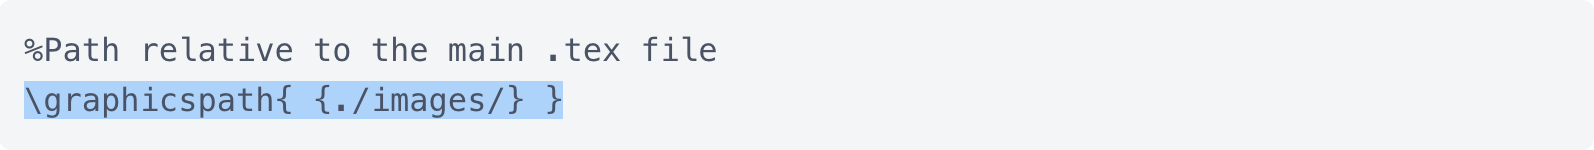
\includegraphics[width=\textwidth]{1.png}
\begin{note}
\textbf{Capital Letters refer to the accelerating reference frame \textit{S} while lowercase letters refer to the inertial reference frame S$_0$}
\end{note}
Picture a moving reference frame, \textit{S}, moving relative to S$_0$. Imagine in the the moving reference frame that a ball with mass, \textit{m} is being thrown. 
In order to consider the motion of the ball, the motion must be first considered in the inertial reference frame. 
\begin{equation}
F = m\ddot{r_0}
\end{equation}
Where r$_0$ is the ball's position relative to S$_0$. 

Now, by considering the motion of the ball in the accelerating frame, the ball position relative to \textit{S} is \textit{R}. (It's velocity is $\dot{R}$. 
Thus, relating \textit{R} to $r_0$, we have: 
\begin{equation}
\dot{r_0} = \dot{R} + V
\end{equation}
Newton's second law for the inertial reference frame by differentiate and multiplying by mass is:
\begin{equation}
F_{\text{inertial}} = -mA = -m\ddot{R}
\end{equation}
\subsection{The Tides}
\begin{shaded}
\textbf{The Tidal Force} \newline
\begin{equation}
F_{tide} = -GM_mm(\frac{\hat{d}}{d^2}-\frac{\hat{d_0}}{d_0^2})
\end{equation}
Where:
\begin{equation*}
\begin{split}
G = \text{Gravitational Constant} \\
d = \text{Object's Position Relative to Moon} \\
d_0 = \text{Earth's Center Relative to the moon}\\
M_m = \text{Mass of the moon}
\end{split}
\end{equation*}
\end{shaded}
\newpage
\subsection{The Angular Velocity Vector}
The rest of the notes and the chapter will over reference frames that are rotating with respect to the inertial reference frame, so angular velocity has to be used. 
\begin{defn}
\textbf{Euler's Theorem} - The most general motion of any body relative to a fixed point \textit{O} is a rotation about some axis through \textit{O} To specify this rotation about a given point O, we only have to give the direction of the axis and the rate of rotation, or angular velocity $\omega$. Because this has a magnitude and direction, it is an obvious choice to write this rotation vector as $\omega$, the angular velocity vector. That is:
\begin{equation}
\omega = \omega\textbf{u}
\end{equation}
Where \textbf{u} is the unit vector
\end{defn}
\begin{shaded}
\textbf{Vector Velocity}\newline
The velocity at any point, \textit{P} (position, \textit{r}) is given by:
\begin{equation}
v = \omega\  x \ r
\end{equation}
\end{shaded}
\subsection*{Addition of Angular Velocities}
One can add angular velocities just like linear velocities. If body 3 is rotating at angular velocity $\omega_{32}$ relative to frame 2, and frame 2 is rotating at angular velocity $\omega_{21}$ relative to frame 1, then body 3 is rotating relative to frame 1 at angular velocity: 
\begin{equation}
\omega_{31} = \omega_{32} + \omega_{21}
\end{equation}
\subsection{Time Derivatives in Rotating Frames}
If frame S has a angular velocity, $\Omega$ relative to S$_0$ then the time derivative of a single vector \textbf{Q} as seen in the two frames are related by:
\begin{equation}
(\frac{d\textbf{Q}}{dt})_{S_0} = (\frac{d\textbf{Q}}{dt})_{S} \ + \Omega \ x \ \textbf{Q}
\end{equation}
\subsection{Netwon's Second Law in a Rotating Frame}
A particle in an inertial reference frame, S$_0$ obeys Newton's second law as we are use to:
\begin{equation}
m\frac{d^2r}{dt^2} = F
\end{equation}
Using the results from equation 8, the time derivative for a rotating frame with reference to an inertial frame can be given by:
\begin{equation}
(\frac{dr}{dt})_{S_0} = (\frac{dr}{dt})_s \ + \Omega \ x \ r
\end{equation}
By differentiation, Newton's second law becomes:
\begin{equation}
m\ddot{r} = F + 2m\dot{r} \ x \ \Omega \ + m(\Omega \ x \ r) \ x \ \Omega
\end{equation}
Where \textit{F} is the sum of all forces in the inertial reference frame. 
\subsection{The Centrifugal Force}
This is an inertial force in a rotating reference frame 
\begin{equation}
F_{\text{cf}} = m(\Omega \ x \ r) \ x \ \Omega
\end{equation}
\subsubsection*{Free-Fall Acceleration (Non-Vertical Gravity)}
\begin{equation}
F_{\text{eff}} = F_{\text{grav}} + F_{\text{cf}} = mg_0 + m\Omega^2R\sin(\theta)\hat{\rho}
\end{equation}
The acceleration due to the Centrifugal force is simply 
\begin{equation}
\begin{split}
g = g_0 + \Omega^2R\sin(\theta)\hat{\rho} \\
g_{\text{rad}} = g_0 - \Omega^2R\sin^2(\theta)  \\
g_{\text{tan}} = \Omega^2R\sin(\theta)\cos(\theta)
\end{split}
\end{equation}
The angle between g and its radial direction is:
\begin{equation}
\alpha \approx \frac{g_{\text{tan}}}{g_{\text{rad}}} 
\end{equation}
The maxium value at ($\theta$ = 45):
\begin{equation}
\alpha_{\text{max}} =  \frac{\Omega^2R}{2g_0}
\end{equation}
\subsection{Coriolis Force}
The Coriolis Force is another inertial force in a rotating reference frame that an object experiences when it is moving. 
\begin{equation}
F_{\text{cor}} = 2m\dot{r} \ x \ \Omega = 2mv \ x \ \Omega
\end{equation}
The maximum acceleration, \textit{a} that the Coriolis force could produce acting by itself with \textit{v} perpendicular to $\Omega$ is:
\begin{equation}
a_{\text{max}} = 2v\Omega 
\end{equation}
\begin{shaded}
\textbf{Direction of the Coriolis Force} \newline
The Direction of the Coriolis force us always perpendicular to the velocity of the object (hence equation 17), and is given by the right hand rule. 
\end{shaded}
\newpage
\subsection{Free Fall and the Coriolis Force}
\begin{equation}
m\ddot{r} = mg_0 + F_{\text{cf}} + F_{\text{cor}} 
\end{equation}
\subsection{The Foucault Pendulum}
See chapter 9, Page 354. There is no need to recopy what is in the book here. 

\end{document}